%% LaTeX Beamer presentation template (requires beamer package)
%% see http://bitbucket.org/rivanvx/beamer/wiki/Home
%% idea contributed by H. Turgut Uyar
%% template based on a template by Till Tantau
%% this template is still evolving - it might differ in future releases!

\documentclass{beamer}

\mode<presentation>
{
\usetheme{Warsaw}

\setbeamercovered{transparent}
%\setbeamercovered{dynamic}
}

\usepackage[english]{babel}
\usepackage[utf8]{inputenc}
\usepackage{graphicx}

\usepackage{booktabs}
\usepackage{hyperref}

%\usepackage[T1]{fontenc}

% More space between rows
\newcommand{\ra}[1]{\renewcommand{\arraystretch}{#1}}

\graphicspath{{./images/}}

%\setbeamertemplate{caption}[numbered]


% font definitions, try \usepackage{ae} instead of the following
% three lines if you don't like this look
\usepackage{mathptmx}
%\usepackage[scaled=1.0]{helvet}
%\usepackage{courier}

\setbeamertemplate{navigation symbols}{}

 \setbeamersize{text margin right=15pt, text margin left=15pt}
\newenvironment{changemargin}[2]{% 
  \begin{list}{}{% 
    \setlength{\topsep}{0pt}% 
    \setlength{\leftmargin}{#1}% 
    \setlength{\rightmargin}{#2}% 
    \setlength{\listparindent}{\parindent}% 
    \setlength{\itemindent}{\parindent}% 
    \setlength{\parsep}{\parskip}% 
  }% 
  \item[]}{\end{list}} 

\title[The Wavelet Trie]{The Wavelet Trie: Maintaining an Indexed Sequence of
Strings in Compressed Space}

\subtitle{CSI 5335 Paper presentation}

% - Use the \inst{?} command only if the authors have different
%   affiliation.
%\author{F.~Author\inst{1} \and S.~Another\inst{2}}
\author[Roberto Grossi, Giuseppe Ottaviano]{{\bf Roberto Grossi, Giuseppe
Ottaviano}\\
presented by: Petr Praus}

\date{April 26th, 2012}


% This is only inserted into the PDF information catalog. Can be left
% out.
%\subject{Talks}



% If you have a file called "university-logo-filename.xxx", where xxx
% is a graphic format that can be processed by latex or pdflatex,
% resp., then you can add a logo as follows:

% \pgfdeclareimage[height=0.5cm]{university-logo}{university-logo-filename}
% \logo{\pgfuseimage{university-logo}}



% Delete this, if you do not want the table of contents to pop up at
% the beginning of each subsection:
%\AtBeginSubsection[]
%{
%\begin{frame}<beamer>
%\frametitle{Outline}
%\tableofcontents[currentsection,currentsubsection]
%\end{frame}
%}

% If you wish to uncover everything in a step-wise fashion, uncomment
% the following command:

%\beamerdefaultoverlayspecification{<+->}

\begin{document}

\section{Problem}

\begin{frame}
\frametitle{Problem}
\begin{itemize}
  \item A lot of things are string sequences
  \item Column databases store and index string sequences
  \item {\bf Great example: access logs}
\end{itemize}
\vspace{10pt}
{\scriptsize
188.26.52.117 - - [24/Apr/2013:03:35:48 -0500] "GET /img/welcome/corner.png\\
188.26.52.117 - - [24/Apr/2013:03:35:49 -0500] "GET /img/welcome/arrowDown.gif\\
188.26.52.117 - - [24/Apr/2013:03:35:49 -0500] "GET /img/welcome/regionals.jpg\\
}
\vspace{10pt}
\begin{changemargin}{-15pt}{-15pt}
\begin{itemize}
  \item Pretty similar, right?
  \item I heard indexes make stuff faster $\rightarrow$ \textbf{indexed sequence of strings}
  \item Rank query: Number of requests for \texttt{/img/welcome/corner.png}?
  \item Select query: Position of $i$-th occurrence of \texttt{/img/welcome/corner.png}
  \item We can do prefix operations too
\end{itemize}
\end{changemargin}
\end{frame}

\begin{frame}
\titlepage
\end{frame}


\section{Building blocks}

\begin{frame}
\frametitle{Patricia Trie}
\begin{itemize}
  \item {\bf Trie} is ordered tree data structure used to store a \emph{dynamic set}
  \item Space-efficient trie
  \item Node always has at least two children
\end{itemize}
\begin{figure}
\scalebox{1.0}{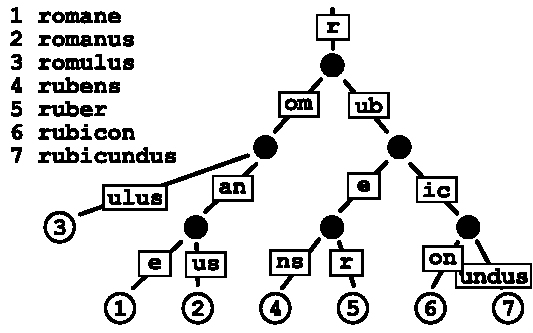
\includegraphics{Patricia_trie.pdf}}
\end{figure}
\end{frame}


\begin{frame}
\frametitle{Wavelet Tree}
\begin{itemize}
  \item Organizes a string into a balanced binary tree of bit vectors
  \item Alphabet $\sum = \{a,b,c,d,r\} \rightarrow \{0, 0, 1, 1, 1\}$
  \item At root, we have \emph{ambiguity}, reducing ambiguity towards leaves
  \item Only the binary vectors are stored!
\end{itemize}
\begin{figure}
\scalebox{0.75}{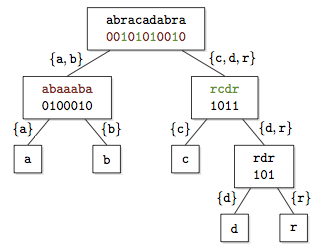
\includegraphics{Wavelet_tree.png}}
\end{figure}
\end{frame}


\begin{frame}
\frametitle{Efficient Computation of Rank in Wavelet Tree}
\begin{itemize}
  \item $rank(8, a)$ = how many a's before position 8
  \item $rank_{bin}(pos, s)$ binary rank, \# of occurences of $s$ before $pos$  
\end{itemize}
\begin{figure}
\scalebox{0.6}{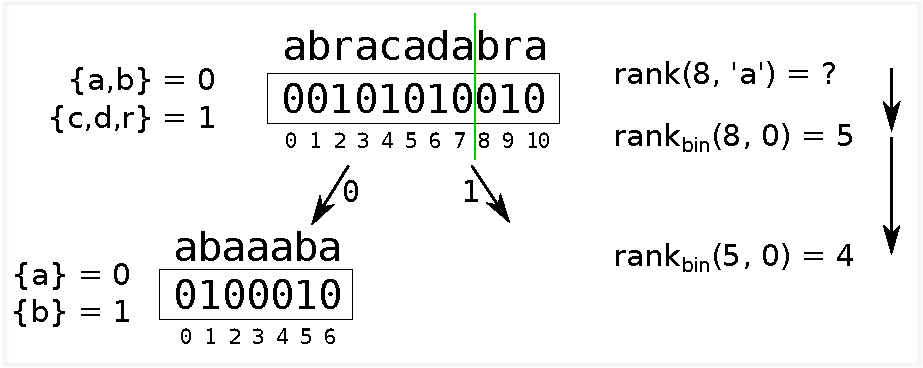
\includegraphics{wavelet_rank.pdf}}
\end{figure}
{\small E.g.: \# of requests to \texttt{/img/welcome/corner.png} before April 10th.}
\end{frame}


\begin{frame}
\frametitle{Mutable \& Compressed Indexed Sequences}
\begin{itemize}
  \item Sequences can change over time:\\$Insert(s, pos)$, $Append(s)$, $Delete(pos)$
  \item Alphabet not always known in advance 
\end{itemize}
\vspace{10pt}
\begin{itemize}
  \item Traditional approach, store explicitly (e.g. array), make an index
  \item Space-inefficient, we want to query the compressed representation
  \item {\bf Succint data structure} -- uses space close to lower information-theoretic bound
\end{itemize}
\vspace{10pt}
\hspace{10pt}
Wavelet Trie to rescue!
\end{frame}


\begin{frame}
\frametitle{Wavelet Trie}
\begin{itemize}
  \item Wavelet Tree + Patricia Trie
  \item Compressed data structure
  \item Can support \emph{Insert}, \emph{Append}, \emph{Delete}, and dynamic alphabet
  \item Variants: Static, Append-only, Fully-dynamic
  \item Note $O(|s|+h_s)$ is very fast for balanced trees
\end{itemize}
\begin{table}[h]
    \centering
    \ra{1.3}
    \resizebox{\columnwidth}{!}{%
    \begin{tabular}{@{}lccccc@{}}
    %\toprule
                    & Query & Append & Insert & Delete  & Space \\
    \midrule
    Static          & $O(|s|+h_s)$ & --      & --      & --       & $LB+o(\tilde{h}n)$ \\
    Append-only     & $O(|s|+h_s)$ & $O(|s|+h_s)$  &   --    & --      & $LB+PT+o(\tilde{h}n)$ \\
    Fully-dynamic   & $O(|s|+h_s \log n)$ & $O(|s|+h_s \log n)$ & $O(|s|+h_s \log n)$ & $O(|s|+h_s \log n)$ & $LB+PT+O(nH_0)$ \\
    \bottomrule
    \end{tabular}
    }
\end{table}
{\small
$h_s$ -- number of nodes traversed while searching for $s$ is Patricia Tree\\
$\tilde{h}$ -- average height of the Wavelet Trie\\
$|s|$ -- length of query string\\
$LB$ -- lower bound on storing the unique elements of a sequence 
}
\end{frame}


\begin{frame}
\frametitle{Wavelet Trie - Example (Static)}
\begin{itemize}
  \item $\sum = \{0001, 0011, 0100, 00100\}$, $\alpha$ common prefix, $\beta$ bit-vector
  \item Splitting based on common prefix like in Patricia Trie, not halving an alphabet like in Wavelet Tree!
\end{itemize}
\begin{figure}[b!]
\scalebox{1.0}{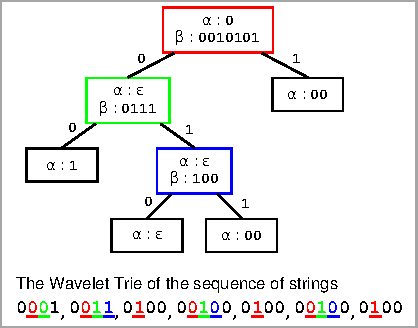
\includegraphics{Wavelet_Trie_example.pdf}}
\end{figure}
\end{frame}


\begin{frame}
\frametitle{Wavelet Trie - Example (Static)}
\begin{itemize}
  \item $Rank(6, 0{\bf 1}00) \rightarrow Rank(6, 1) = 2$
  \item Notice how ambiguity decreases towards the leaves
\end{itemize}
\begin{figure}[b]
\scalebox{1.0}{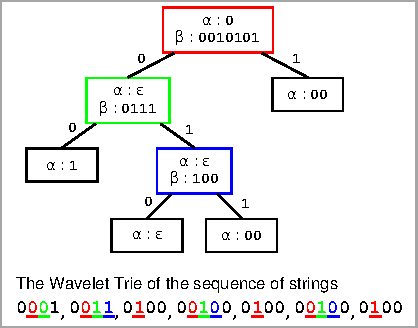
\includegraphics{Wavelet_Trie_example.pdf}}
\end{figure}
\end{frame}


\begin{frame}
\frametitle{Dynamic Wavelet Tries}
\begin{itemize}
  \item Bitvectors must support insertion and deletion
  \item We also want dynamic alphabet, e.g. we want to add ``0111'' 
\end{itemize}
\begin{figure}[b]
\scalebox{0.9}{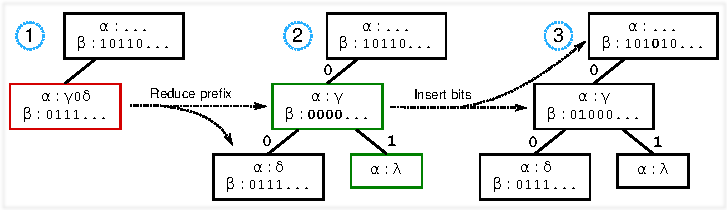
\includegraphics{Wavelet_Trie_insert.pdf}}
\end{figure}
Inserting new $s = \ldots\gamma 1 \lambda$ at $pos=3$; $\gamma$ -- common prefix, $\lambda$ -- suffix
\begin{enumerate}
  \item Original Wavelet Trie
  \item After splitting red node, adding internal node and leaf node (green)
  \item Inserting bits in the root-to-leaf path nodes
\end{enumerate}
\end{frame}

\begin{frame}
\frametitle{Summary}
\begin{itemize}
  \item Wavelet Trie = Wavelet Tree + Patricia Trie
  \item Compressed sequences of strings
  \item Very space efficient (no need for data+index)
  \item Applications in column databases, access log aggregation, \ldots
  \item Quite fast, querying in $O(|s|+h_s)$
  \item Can support prefix searches
\end{itemize}
\end{frame}

\begin{frame}
\frametitle{}
\begin{center}
\large \bf Thank you.
\end{center}
\end{frame}
 
\begin{frame}
\frametitle{Resources}
\begin{itemize}
  \item Grossi, Roberto, and Giuseppe Ottaviano. ``The wavelet trie: Maintaining an indexed sequence of strings in compressed space.'' In Proceedings of the 31st symposium on Principles of Database Systems, pp. 203-214. ACM, 2012.
  \item \url{http://alexbowe.com/wavelet-trees/}
  \item \url{http://en.wikipedia.org/wiki/Wavelet_Tree}
  \item \url{http://siganakis.com/challenge-design-a-data-structure-thats-small}
\end{itemize}
\end{frame}
 
 

%\begin{frame}
%\frametitle{}

% You can create overlays
% \begin{itemize}
%   \item using the \texttt{pause} command:
%   \begin{itemize}
%     \item First item.
%     \pause
%     \item Second item.
%   \end{itemize}
%   \item using overlay specifications:
%   \begin{itemize}
%     \item<3-> First item.
%     \item<4-> Second item.
%   \end{itemize}
%   \item using the general \texttt{uncover} command:
%   \begin{itemize}
%     \uncover<5->{\item First item.}
%     \uncover<6->{\item Second item.}
%   \end{itemize}
% \end{itemize}
% \end{frame}
% 
% \section*{Summary}
% 
% \begin{frame}
% \frametitle<presentation>{Summary}
% 
% \begin{itemize}
%   \item The \alert{first main message} of your talk in one or two lines.
% \end{itemize}
% 
% % The following outlook is optional.
% \vskip0pt plus.5fill
% \begin{itemize}
%   \item Outlook
%   \begin{itemize}
%     \item Something you haven't solved.
%     \item Something else you haven't solved.
%   \end{itemize}
% \end{itemize}
% \end{frame}
% 
% \end{document}
